%!TEX root = /Users/nebolsin/Documents/MSU/Graduate Work/tex/main.tex

\section{Разработка архитектуры распределенной вычислительной среды}
\label{research}

В данном разделе описывается архитектура распределенной вычислительной среды, предназначенной для высокоуровневого решения проблем. Сначала рассматриваются исходные данные и требования к системе, после чего строится адекватная описанным требованиям архитектура.

\subsection{Исходные данные для вычислительной среды}

Исходными данными для работы вычислительной среды являются существующие компоненты и модели, а также данные, подлежащие обработке.

Компонентом среды может являться как исходный код, предназначенный для компиляции и запуска на различных вычислительных узлах, так и установленный на конкретном вычислительном узле сложный программный (или программно-аппаратный) паккет или библиотека. Пользователь должен иметь возможность запуска таких компонентов на вычисление и получение результата.

Модель отражает последовательность действий, которые необходимо провести для решения поставленной задачи. В рамках среды модель --- это ориентированный граф из компонентов. Например, если необходимо посчитать квадрат суммы двух матриц, а в нашем распоряжении имеются отдельные компоненты для вычисления суммы и произведения двух матриц, то модель будет иметь вид простого графа, представленного на рис.~\ref{fig:model-graph}

\begin{figure}
  \centering
    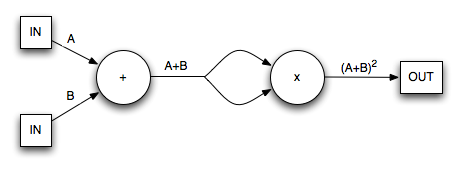
\includegraphics[width=8cm]{images/model-graph.png}
  \caption{Пример графа модели для решения задачи о нахождении квадрата суммы двух матриц.}
  \label{fig:model-graph}
\end{figure}  

Входные данные, это просто файлы с данными, которые пользователю необходимо подать на вход той или иной модели или компоненту.
                                 
Таким образом, для того, чтобы вычислительную среду возможно было использовать, в ней должны поддерживаться адекватные представления для компонентов, моделей и файлов с входными данными.

\subsection{Представление компонентов}  

Как показано в разделе~\ref{intro} и проиллюстрировано многочисленными примерами в разделе~\ref{review}, удобство взаимодействия ученого с системой прямо связано с адекватностью реализованного в системе представления компонентов. Хотя и верно, что ни одно универсальное представление не может быть идеальным для всех целей, традиционных подходов, применяемых в Grid проектах (для представления моделей, экземпляров моделей и имитаций), не достаточно для поддержки высокоуровневого решения задач.

В разделе~\ref{architecture} модель определяется как ориентированный граф отдельных вычислительных кодов или запускаемых приложений. Понятие <<представление модели>> допускает многочисленные интерпретации и интенсивно обсуждается в литературе о моделировании (например, XXX). Введем определение представления модели, а именно, что представление модели --- это такая абстракция модели, которая допускает применение при высокоуровневом решении задач, которое не было бы возможным при использовании модели как таковой. Эта абстракция может отражать функциональное поведение модели, структурную организацию модели, профиль производительности, связь с другими моделями и/или информацию о том, как данная модель может быть включена в вычислительный контекст РВС и какие функции она может выполнять.

Рассмотрим два экстремальных примера представления одного вычислительного компонента (простейшей модели) в РВС. В варианте <<черный ящик>> в качестве представления модели используется только ее название. Такое решение очень хорошо подходит при ссылках на компонент (например, <<запустить компонент X>>), но совершенно не подходит для более детального изучения компонента (например, <<является ли X итеративным алгоритмом>>). Другим экстремальным вариантом является вариант <<белый ящик>>, при котором компонент сам выступает в качестве своего представления (например, математическое описание научного феномена). Обычно в таких случаях представление компонентов связано с теориями и алгоритмами из предметной области. Несмотря на огромный потенциал таких представлений, они подходят только для ограниченного применения. 

Предлагаемое решение состоит в том, что представлением компонента (модели) является его название и аннотации в виде пар (функция, значение), описывающих дополнительные свойства компонента. Например, такие аннотации могут включать директивы и флаги, необходимые для компиляции кода на конкретной платформе. 

\subsection{Подсистема управления данными}

Работа с данными является ключевым звеном при решении научных вычислительных задач. Для работы практически всех компонентов необходимы входные данные и абсолютно все компоненты производят выходные данные (в противном случае работа компонента не будет иметь смысла). Кроме того, при проведении некоторых вычислений могут образовываться промежуточные данные, которые не требуются в данном конкретном эксперименте, но могут быть использованы впоследствии. Это показывает важность правильной организации подсистемы управления данными в распределенной вычислительной среде.

 

\subsection{Выполнение вычислений}

\subsection{Организация межпользовательского взаимодействия}